%*******10********20********30********40********50********60********70********80
\clearpage
\subsection{Expansion Intensified Part Range Related to Behavior of Concrete During DEF Expansion}




\begin{figure}[!ht]
\centering
    %*******
    \begin{subfigure}{.33\textwidth}
      \centering
      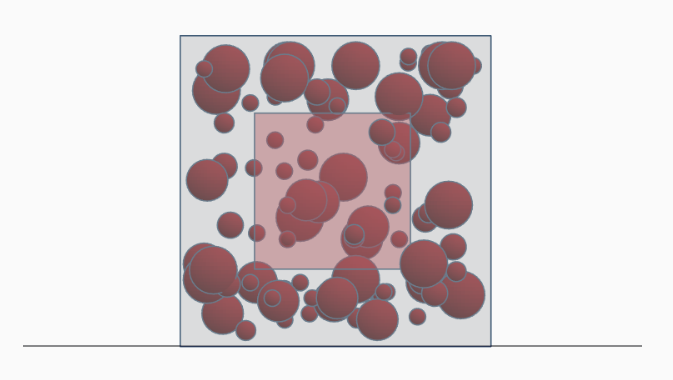
\includegraphics[width=.8\linewidth]{Files/DEF_X/X0_3ds.png}
      \caption{Intensified 50x50x50mm Case\\ Cross Section}
    \end{subfigure}%
    %*******
    \begin{subfigure}{.33\textwidth}
      \centering
      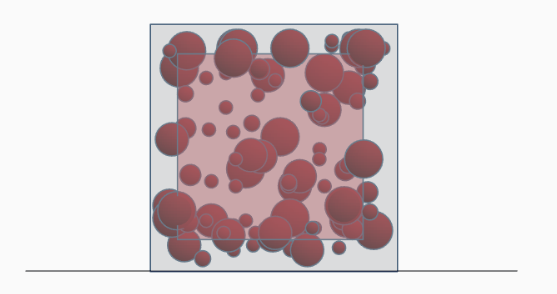
\includegraphics[width=.8\linewidth]{Files/DEF_X/X-5_3ds.png}
      \caption{Intensified 75x75x75mm Case \\ Cross Section}
    \end{subfigure}%
    %*******
    \begin{subfigure}{.33\textwidth}
      \centering
      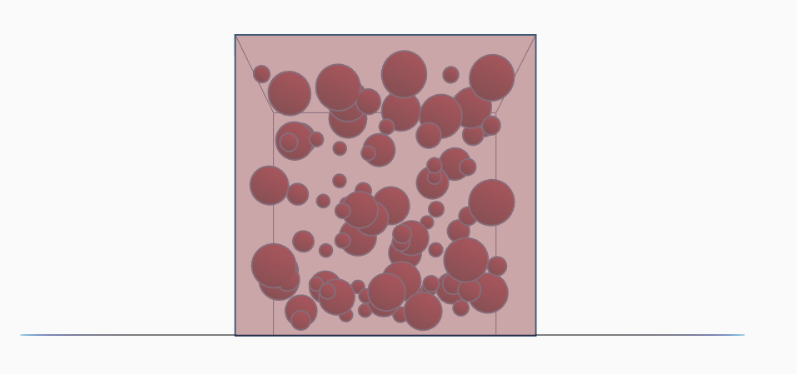
\includegraphics[width=.9\linewidth]{Files/DEF_X/X-1_3ds.png}
      \caption{Intensified 100x100x100mm Case\\ Cross Section}
    \end{subfigure}
    %*******
  \caption{DEF intensified part range}
  \label{fig:DEF_X}
\end{figure}

In this section, DEF expansion simulation result of intensified center 75x75x75mm and uniformly expansion for all part (intensified center 100x100x100mm) is presented.

\subsubsection{Expansion Intensified 75x75x75mm at Center of Model}

\begin{table}[ht!]
\centering
\begin{tabular}{ ||p{2cm}|p{2cm}|p{2cm}| }
 \hline
    Initial Strain (Each Step) & Expanding Steps &  Final Expansion[\%] \\ [0.5ex]
 \hline\hline
  0 & 0 & 0  \\
  0.001 & 20 & 0.1671 \\
  0.002 & 20 & 0.3380 \\
  0.003 & 20 & 0.5118 \\
  0.005 & 20 & 0.8577 \\
 \hline
\end{tabular}
\caption{One Dimensional Expansion Ratio in Expansion Intensified 75x75x75mm at Center of Model DEF Model Simulation}
\label{table:DEF_X-5_EXP}
\end{table}

\begin{figure}[ht!]
\centering
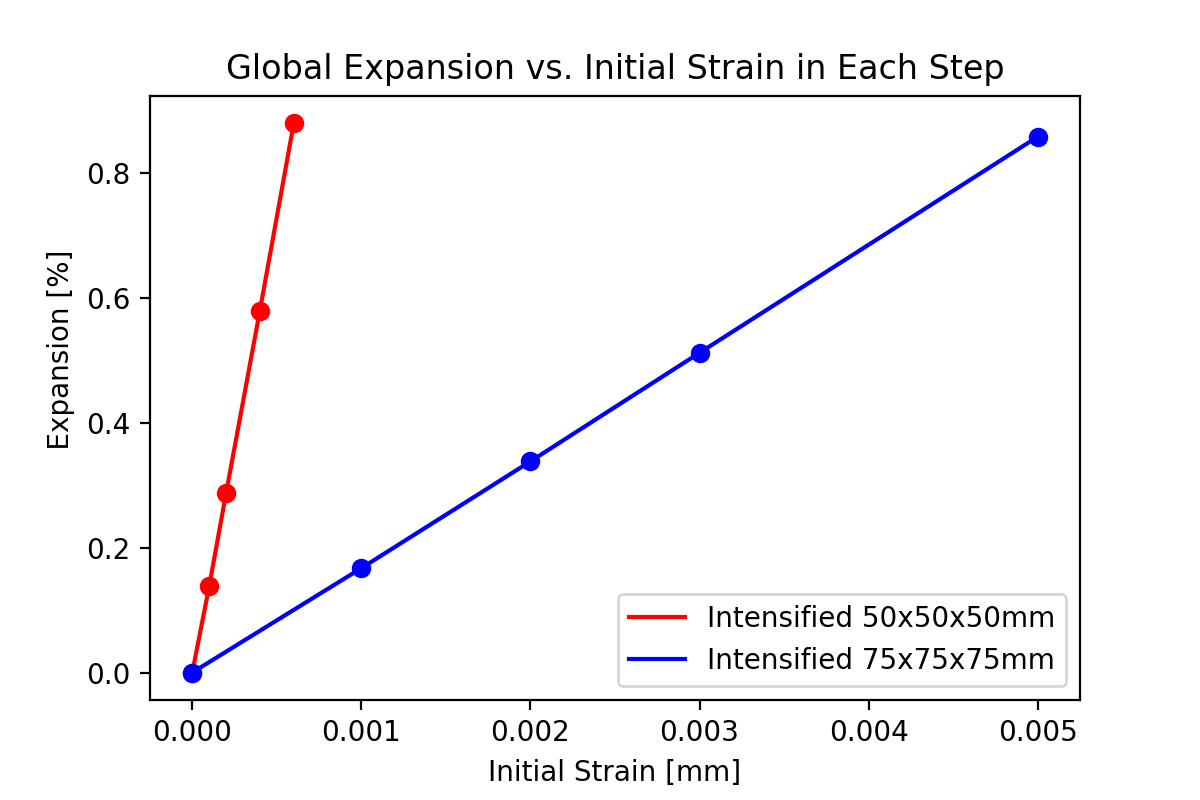
\includegraphics[width=.8\linewidth]{Files/exp_plot/DEFA30X0vsX-5_exp.png}
  \caption{Global Expansion vs. Step}
  \label{fig:DEFA30X0vsX-5_exp}
\end{figure}

% Surface
\begin{figure}[!h]
\centering

    %*******
    \begin{subfigure}{.5\textwidth}
      \centering
      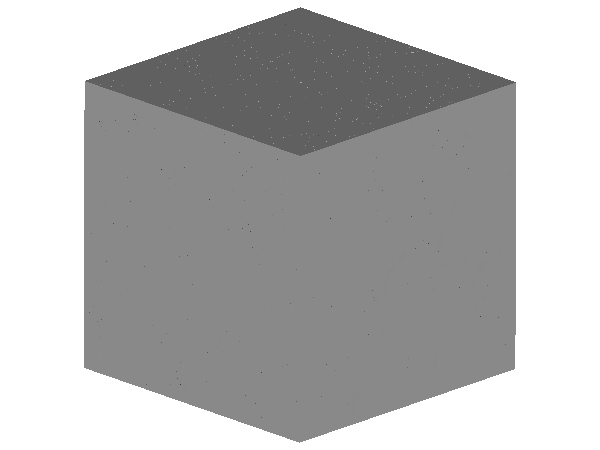
\includegraphics[width=.8\linewidth]{Files/exp_3D/ASR/A30Undamaged.png} %TODO: Fix. Should be A30
    \caption{Case 0: 0\% Expansion}
    \end{subfigure}%
    %*******
    \begin{subfigure}{.5\textwidth}
      \centering
      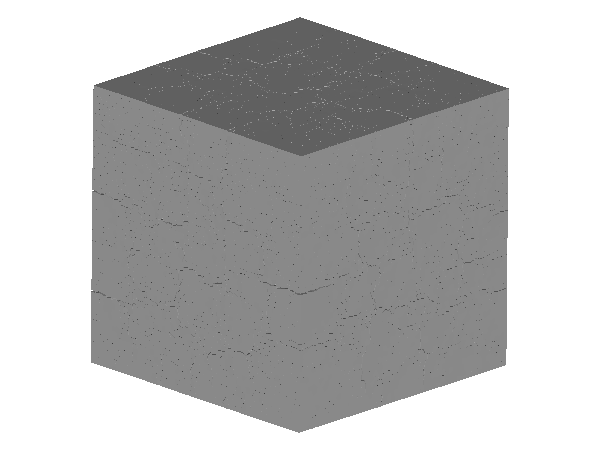
\includegraphics[width=.8\linewidth]{Files/exp_3D/DEF/A30X-5C_1_3d.png}
    \caption{Case 1: 0.1671\% Expansion}
    \end{subfigure}
    %*******
    \begin{subfigure}{.5\textwidth}
      \centering
      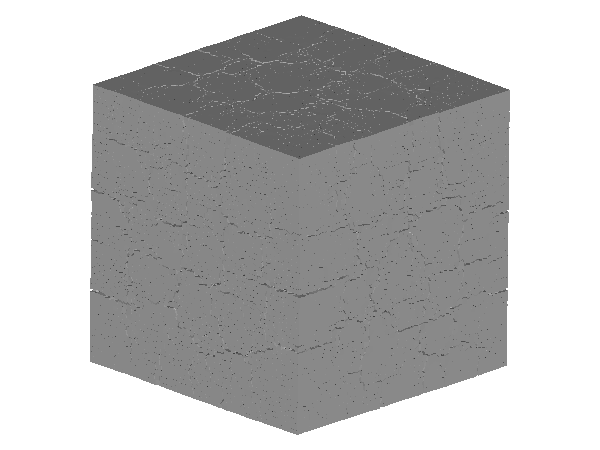
\includegraphics[width=.8\linewidth]{Files/exp_3D/DEF/A30X-5C_2_3d.png}
    \caption{Case 2: 0.3380\% Expansion}
    \end{subfigure}%
    %*******
    \begin{subfigure}{.5\textwidth}
      \centering
      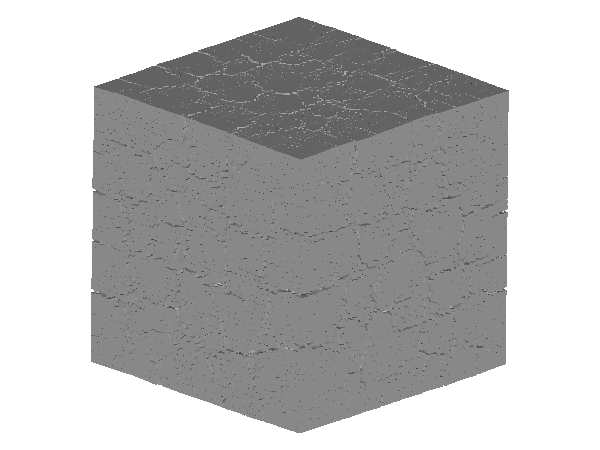
\includegraphics[width=.8\linewidth]{Files/exp_3D/DEF/A30X-5C_3_3d.png}
    \caption{Case 3: 0.5118\% Expansion}
    \end{subfigure}
    %*******
    \begin{subfigure}{.5\textwidth}
      \centering
      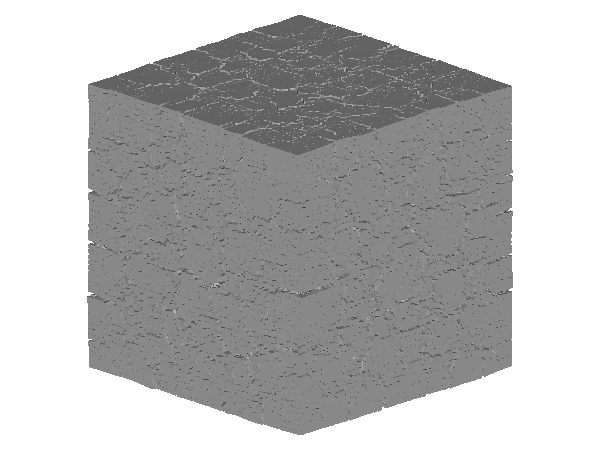
\includegraphics[width=.8\linewidth]{Files/exp_3D/DEF/A30X-5C_4_3d.png}
    \caption{Case 4: 0.8577\% Expansion}
    \end{subfigure}%
    %*******

  \caption{3D Surface Cracks Expansion Intensified 75x75x75mm (Deformation x 10)}
  \label{fig:DEF_A30X-5C_3D}
\end{figure}

% Surface of one side
\begin{figure}[!h]
\centering

    %*******
    \begin{subfigure}{.5\textwidth}
      \centering
      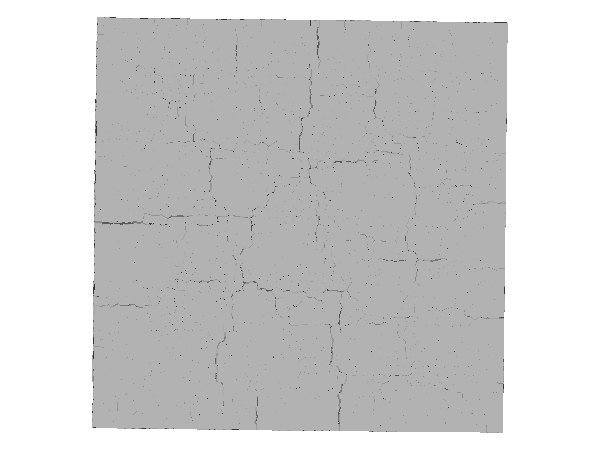
\includegraphics[width=.8\linewidth]{Files/exp_3D/DEF/A30X-5C_1_3ds.png}
    \caption{Case 0: 0\% Expansion}
    \end{subfigure}%
    %*******
    \begin{subfigure}{.5\textwidth}
      \centering
      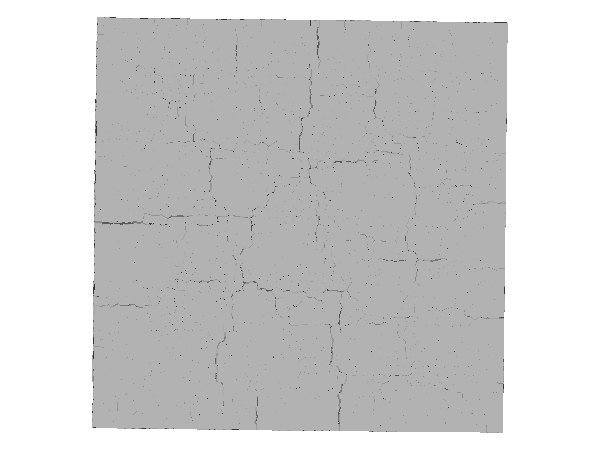
\includegraphics[width=.8\linewidth]{Files/exp_3D/DEF/A30X-5C_1_3ds.png}
    \caption{Case 1: 0.1671\% Expansion}
    \end{subfigure}
    %*******
    \begin{subfigure}{.5\textwidth}
      \centering
      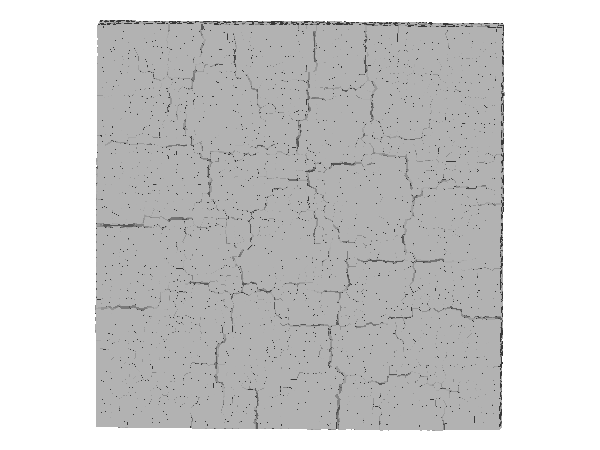
\includegraphics[width=.8\linewidth]{Files/exp_3D/DEF/A30X-5C_2_3ds.png}
    \caption{Case 2: 0.3380\% Expansion}
    \end{subfigure}%
    %*******
    \begin{subfigure}{.5\textwidth}
      \centering
      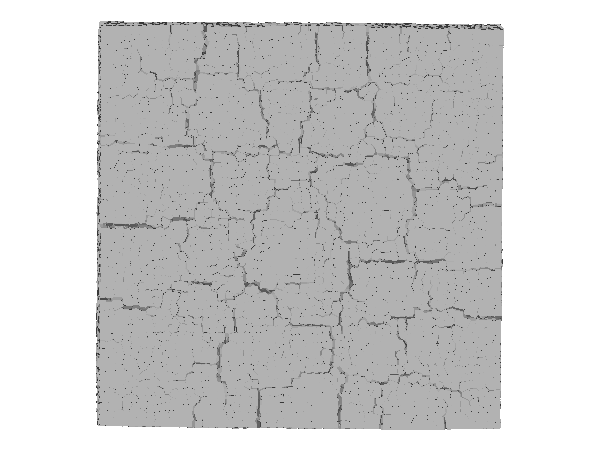
\includegraphics[width=.8\linewidth]{Files/exp_3D/DEF/A30X-5C_3_3ds.png}
    \caption{Case 3: 0.5118\% Expansion}
    \end{subfigure}
    %*******
    \begin{subfigure}{.5\textwidth}
      \centering
      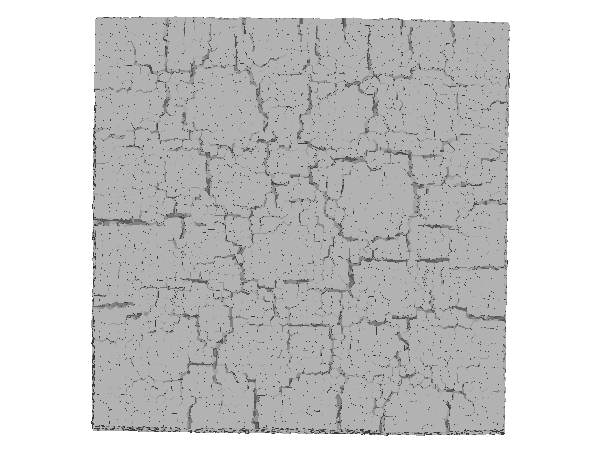
\includegraphics[width=.8\linewidth]{Files/exp_3D/DEF/A30X-5C_4_3ds.png}
    \caption{Case 4: 0.8577\% Expansion}
    \end{subfigure}%

  \caption{3D Surface Cracks (Single Side View) Expansion Intensified 75x75x75mm (Deformation x 10)}
  \label{fig:ASR_A30X-5C_3DS}
\end{figure}

% Inner Crack
\begin{figure}[!h]
\centering

    %*******
    \begin{subfigure}{.5\textwidth}
      \centering
      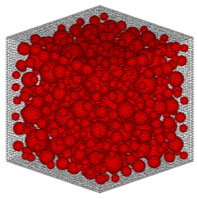
\includegraphics[width=.6\linewidth]{Files/Aggregate/A30.png} %TODO: Fix. Should be A30
    \caption{Case 0: 0\% Expansion}
    \end{subfigure}%
    %*******
    \begin{subfigure}{.5\textwidth}
      \centering
      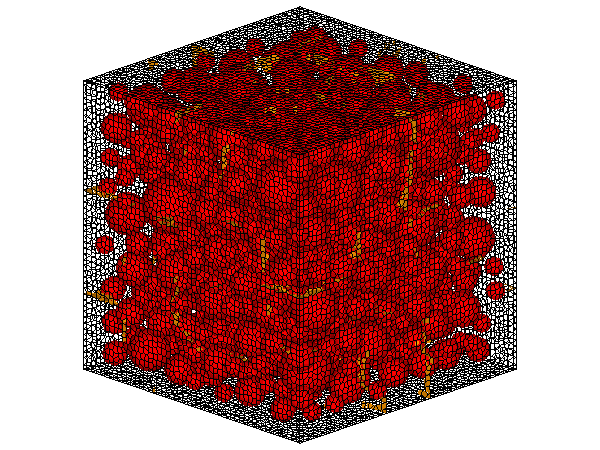
\includegraphics[width=.8\linewidth]{Files/exp_3D/DEF/A30X-5C_1_c.png}
    \caption{Case 1: 0.1671\% Expansion}
    \end{subfigure}
    %*******
    \begin{subfigure}{.5\textwidth}
      \centering
      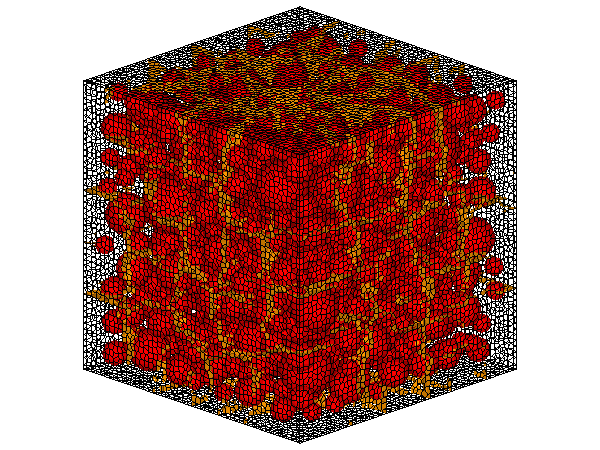
\includegraphics[width=.8\linewidth]{Files/exp_3D/DEF/A30X-5C_2_c.png}
    \caption{Case 2: 0.3380\% Expansion}
    \end{subfigure}%
    %*******
    \begin{subfigure}{.5\textwidth}
      \centering
      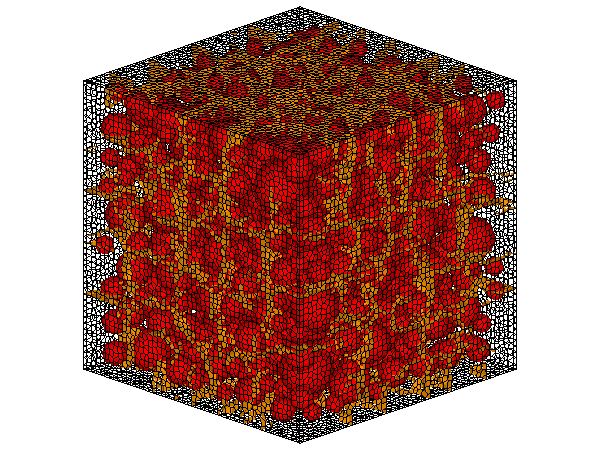
\includegraphics[width=.8\linewidth]{Files/exp_3D/DEF/A30X-5C_3_c.png}
    \caption{Case 3: 0.5118\% Expansion}
    \end{subfigure}
    %*******
    \begin{subfigure}{.5\textwidth}
      \centering
      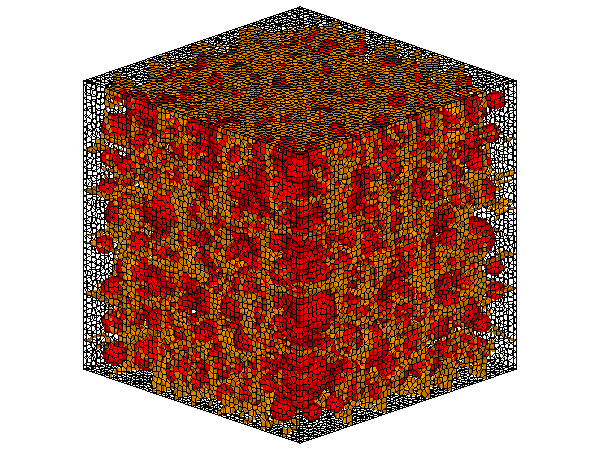
\includegraphics[width=.8\linewidth]{Files/exp_3D/DEF/A30X-5C_4_c.png}
    \caption{Case 4: 0.8577\% Expansion}
    \end{subfigure}%
    %*******

  \caption{3D Inner Cracks Expansion Intensified 75x75x75mm}
  \label{fig:DEF_A30X-5C_3D}
\end{figure}
\subsubsection{Expansion Intensified 100x100X100mm at Center of Model}

\begin{table}[ht!]
\centering
\begin{tabular}{ ||p{2cm}|p{2cm}|p{2cm}| }
 \hline
    Initial Strain (Each Step) & Expanding Steps &  Final Expansion[\%] \\ [0.5ex]
 \hline\hline
  0 & 0 & 0 \\
  0.001 & 20 & 0.2 \\
  0.002 & 20 & 0.4087 \\
  0.004 & 20 & 0.6191 \\
  0.006 & 20 & 1.0454 \\
 \hline
\end{tabular}
\caption{One Dimensional Expansion Ratio in Expansion Intensified 100x100X100mm at Center of Model DEF Model Simulation}
\label{table:DEF_X-1_EXP}
\end{table}

\begin{figure}[ht!]
\centering
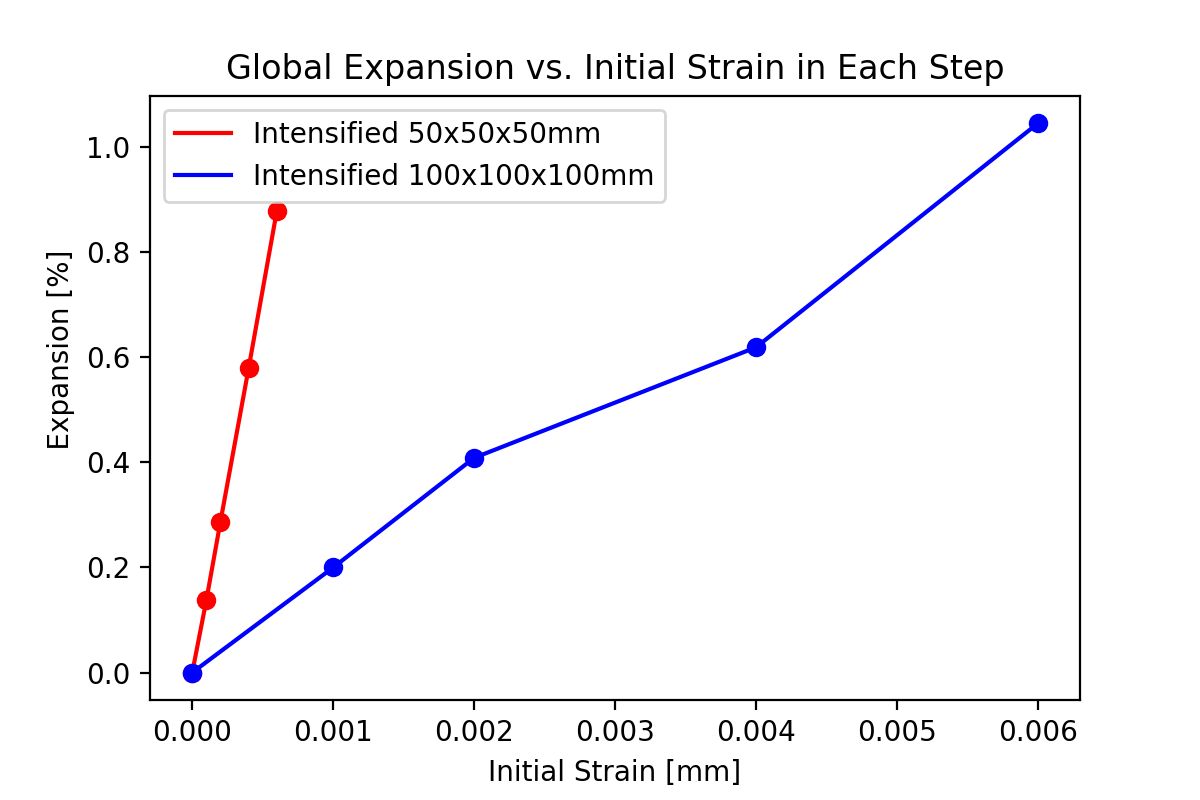
\includegraphics[width=.8\linewidth]{Files/exp_plot/DEFA30X0vsX-1_exp.png}
  \caption{Global Expansion vs. Step}
  \label{fig:DEFA30X0vsX-1_exp}
\end{figure}
\begin{figure}[ht!]
\centering

    %*******
    \begin{subfigure}{.5\textwidth}
      \centering
      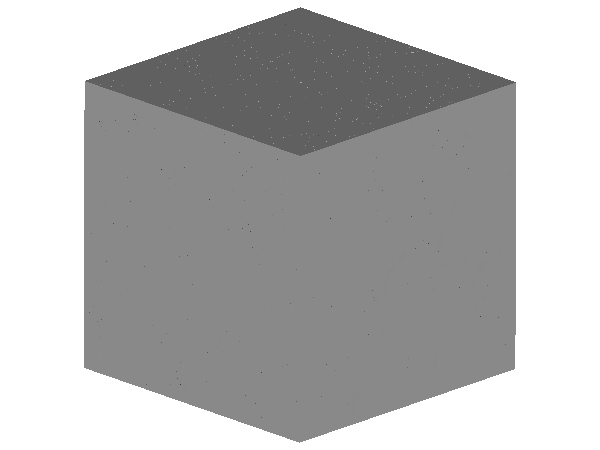
\includegraphics[width=.8\linewidth]{Files/exp_3D/ASR/A30Undamaged.png} %TODO: Fix. Should be A30
    \caption{Case 0: 0\% Expansion}
    \end{subfigure}%
    %*******
    \begin{subfigure}{.5\textwidth}
      \centering
      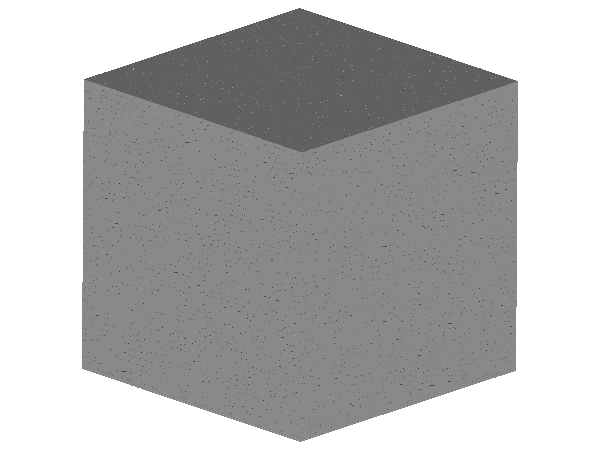
\includegraphics[width=.8\linewidth]{Files/exp_3D/DEF/A30X-1C_1_3d.png}
    \caption{Case 1: 0.2\% Expansion}
    \end{subfigure}
    %*******
    \begin{subfigure}{.5\textwidth}
      \centering
      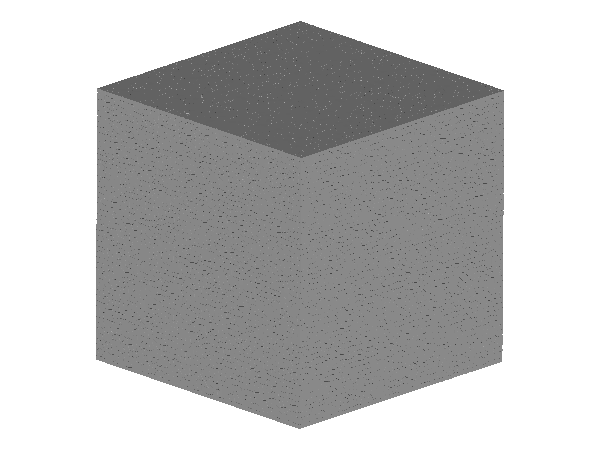
\includegraphics[width=.8\linewidth]{Files/exp_3D/DEF/A30X-1C_2_3d.png}
    \caption{Case 2: 0.4087\% Expansion}
    \end{subfigure}%
    %*******
    \begin{subfigure}{.5\textwidth}
      \centering
      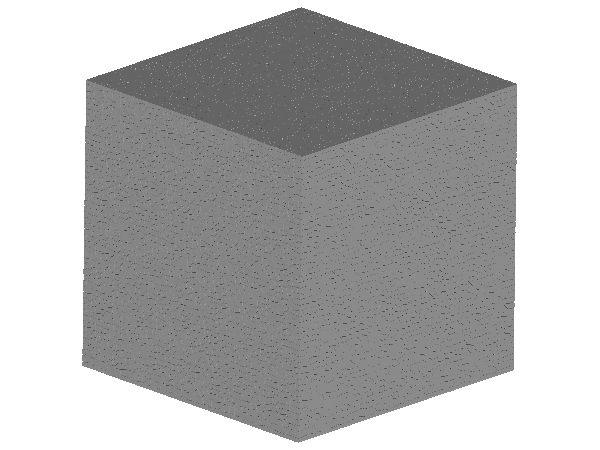
\includegraphics[width=.8\linewidth]{Files/exp_3D/DEF/A30X-1C_3_3d.png}
    \caption{Case 3: 0.6191\% Expansion}
    \end{subfigure}
    %*******
    \begin{subfigure}{.5\textwidth}
      \centering
      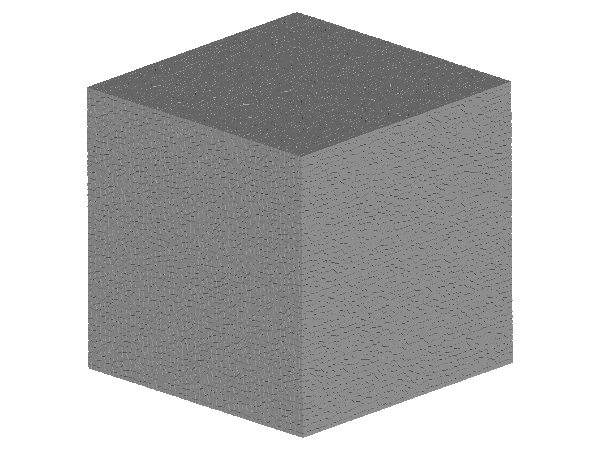
\includegraphics[width=.8\linewidth]{Files/exp_3D/DEF/A30X-1C_4_3d.png}
    \caption{Case 4: 1.0454\% Expansion}
    \end{subfigure}%
    %*******

  \caption{3D Surface Cracks Expansion Intensified 100x100X100mm (Deformation x 10)}
  \label{fig:DEF_A30X-1C_3D}
\end{figure}

% Surface of one side
\begin{figure}[ht!]
\centering

    %*******
    \begin{subfigure}{.5\textwidth}
      \centering
      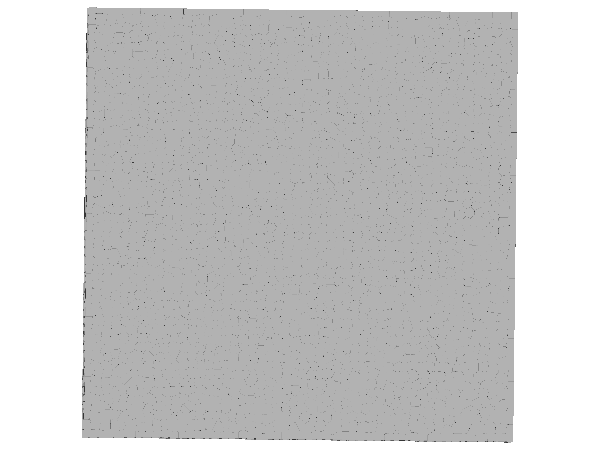
\includegraphics[width=.8\linewidth]{Files/exp_3D/DEF/A30X-1C_1_3ds.png}
    \caption{Case 0: 0\% Expansion}
    \end{subfigure}%
    %*******
    \begin{subfigure}{.5\textwidth}
      \centering
      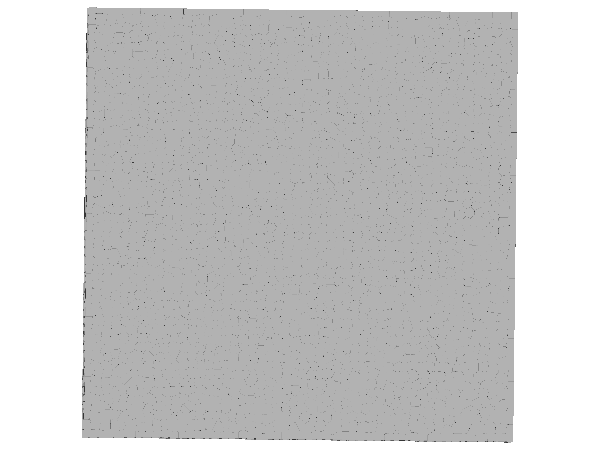
\includegraphics[width=.8\linewidth]{Files/exp_3D/DEF/A30X-1C_1_3ds.png}
    \caption{Case 1: 0.2\% Expansion}
    \end{subfigure}
    %*******
    \begin{subfigure}{.5\textwidth}
      \centering
      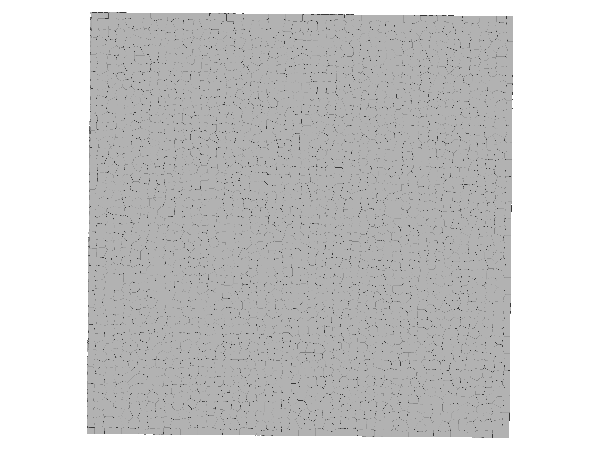
\includegraphics[width=.8\linewidth]{Files/exp_3D/DEF/A30X-1C_2_3ds.png}
    \caption{Case 2: 0.4087\% Expansion}
    \end{subfigure}%
    %*******
    \begin{subfigure}{.5\textwidth}
      \centering
      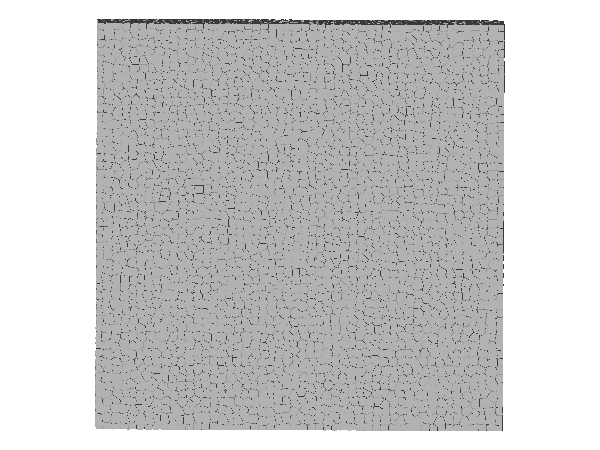
\includegraphics[width=.8\linewidth]{Files/exp_3D/DEF/A30X-1C_3_3ds.png}
    \caption{Case 3: 0.6191\% Expansion}
    \end{subfigure}
    %*******
    \begin{subfigure}{.5\textwidth}
      \centering
      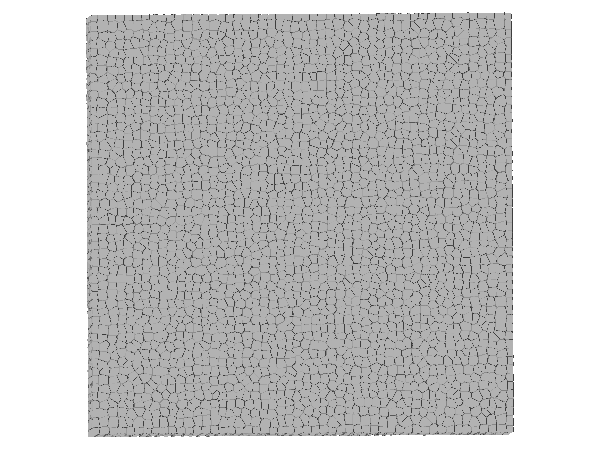
\includegraphics[width=.8\linewidth]{Files/exp_3D/DEF/A30X-1C_4_3ds.png}
    \caption{Case 4: 1.0454\% Expansion}
    \end{subfigure}%

  \caption{3D Surface Cracks (Single Side View) Expansion Intensified 100x100X100mm (Deformation x 10)}
  \label{fig:ASR_A30X-1C_3DS}
\end{figure}

\begin{figure}[ht!]
\centering

    %*******
    \begin{subfigure}{.5\textwidth}
      \centering
      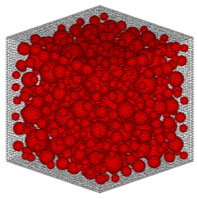
\includegraphics[width=.6\linewidth]{Files/Aggregate/A30.png} %TODO: Fix. Should be A30
    \caption{Case 0: 0\% Expansion}
    \end{subfigure}%
    %*******
    \begin{subfigure}{.5\textwidth}
      \centering
      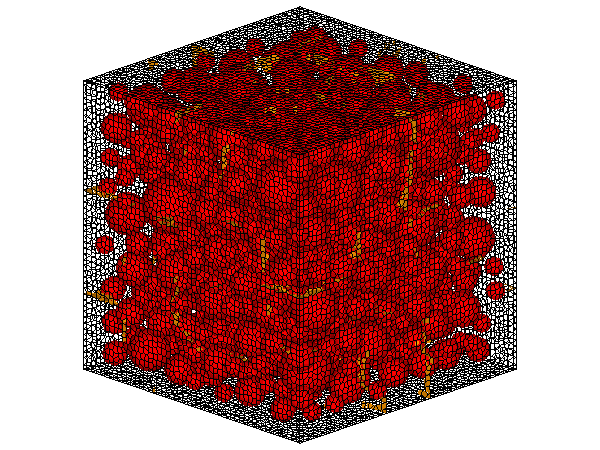
\includegraphics[width=.8\linewidth]{Files/exp_3D/DEF/A30X-1C_1_c.png}
    \caption{Case 1: 0.2\% Expansion}
    \end{subfigure}
    %*******
    \begin{subfigure}{.5\textwidth}
      \centering
      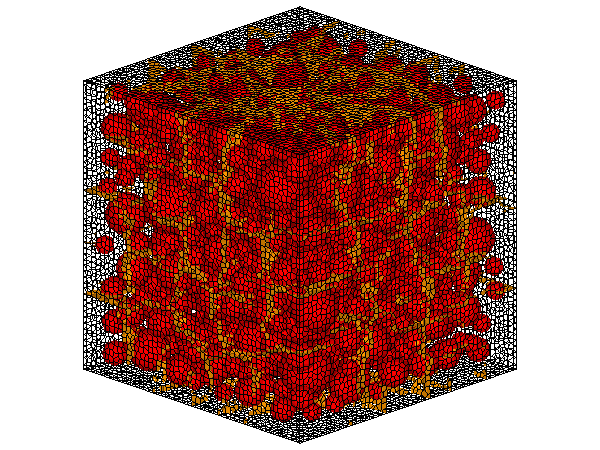
\includegraphics[width=.8\linewidth]{Files/exp_3D/DEF/A30X-1C_2_c.png}
    \caption{Case 2: 0.4087\% Expansion}
    \end{subfigure}%
    %*******
    \begin{subfigure}{.5\textwidth}
      \centering
      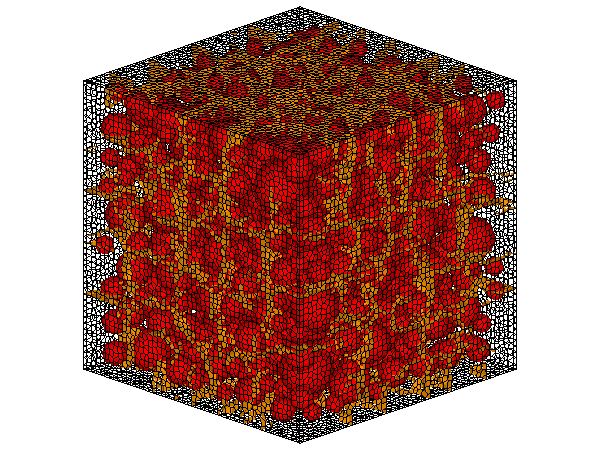
\includegraphics[width=.8\linewidth]{Files/exp_3D/DEF/A30X-1C_3_c.png}
    \caption{Case 3: 0.6191\% Expansion}
    \end{subfigure}
    %*******
    \begin{subfigure}{.5\textwidth}
      \centering
      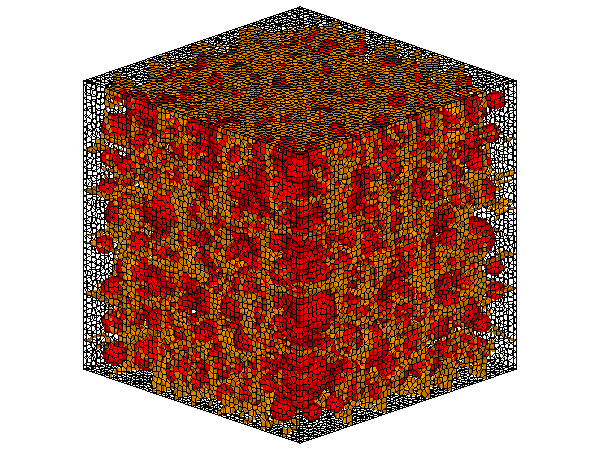
\includegraphics[width=.8\linewidth]{Files/exp_3D/DEF/A30X-1C_4_c.png}
    \caption{Case 4: 1.0454\% Expansion}
    \end{subfigure}%
    %*******

  \caption{3D Inner Cracks Expansion Intensified 100x100X100mm (Deformation x 10)}
  \label{fig:DEF_A30X-1C_3D}
\end{figure}


From Figure \ref{fig:ASR_A30X-5C_3D}, Figure \ref{fig:ASR_A30X-5C_3DS}, Figure \ref{fig:ASR_A30X-1C_3D} and Figure \ref{fig:ASR_A30X-1C_3DS}, it can be seen that when intensified the DEF expansion at the center 75x75x75mm, still the characteristic map cracking pattern can be achieved, which is similar to 50x50x50mm case.

However, when comparing to uniformed overall expansion (DEF expansion at the center 75x75x75mm), the increasing of the concrete volume is achieved without generating significant surface cracks. This simulation result is correlated with the research result done by L.Eddy et.al., 2016, concluded as the simply uniformed paste expansion does not present DEF simulation well as it behaves in reality.

\begin{figure}[ht!]
\centering
    %*******
    \begin{subfigure}{.3\textwidth}
      \centering
      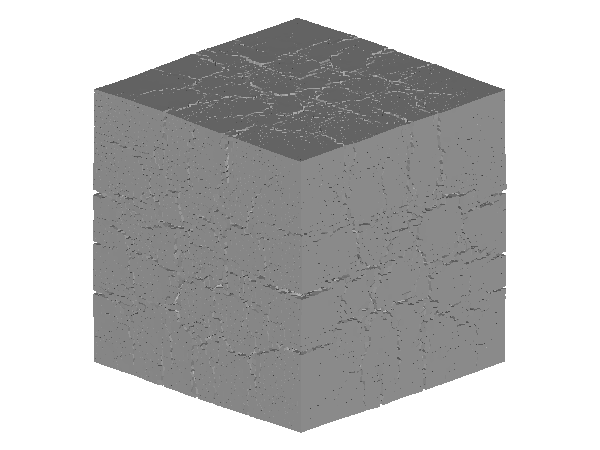
\includegraphics[width=.9\linewidth]{Files/exp_3D/DEF/A30X0C_3_3d.png}
    \caption{Intensified 50x50x50mm \\ 0.5795\% Expansion}
    \end{subfigure}%
    %*******
    \begin{subfigure}{.3\textwidth}
      \centering
      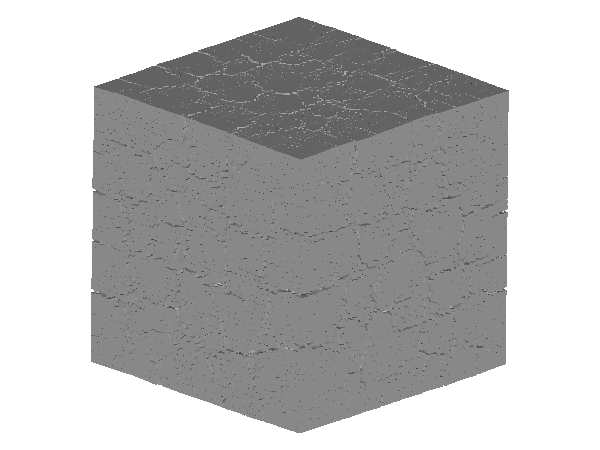
\includegraphics[width=.9\linewidth]{Files/exp_3D/DEF/A30X-5C_3_3d.png}
    \caption{Intensified 75x75x75mm \\  0.5118\% Expansion}
    \end{subfigure}
    %*******
    \begin{subfigure}{.3\textwidth}
      \centering
      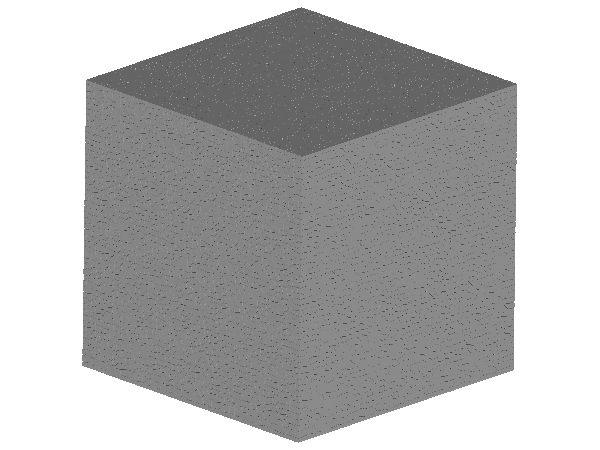
\includegraphics[width=.9\linewidth]{Files/exp_3D/DEF/A30X-1C_3_3d.png}
    \caption{Intensified 100x100x100mm \\  0.6191\% Expansion}
    \end{subfigure}%
    %*******

    %*******
    \begin{subfigure}{.3\textwidth}
      \centering
      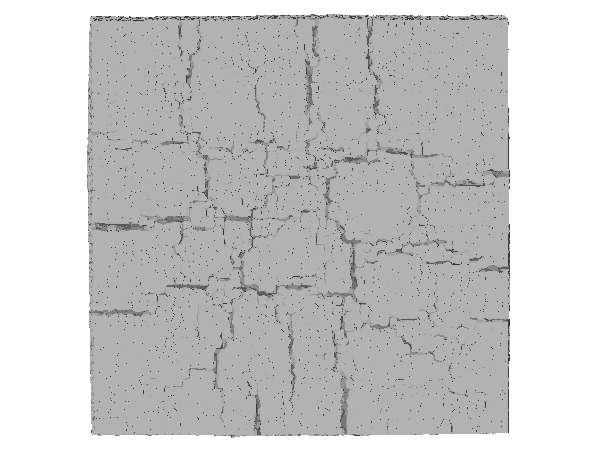
\includegraphics[width=.9\linewidth]{Files/exp_3D/DEF/A30X0C_3_3ds.png}
    \caption{Intensified 50x50x50mm \\  0.5795\% Expansion}
    \end{subfigure}%
    %*******
    \begin{subfigure}{.3\textwidth}
      \centering
      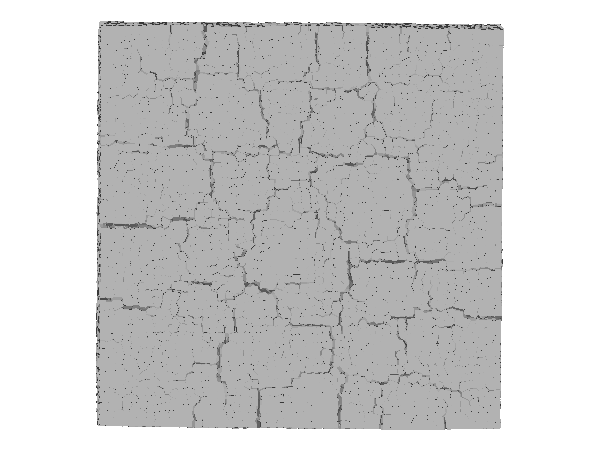
\includegraphics[width=.9\linewidth]{Files/exp_3D/DEF/A30X-5C_3_3ds.png}
    \caption{Intensified 75x75x75mm \\  0.5118\% Expansion}
    \end{subfigure}
    %*******
    \begin{subfigure}{.3\textwidth}
      \centering
      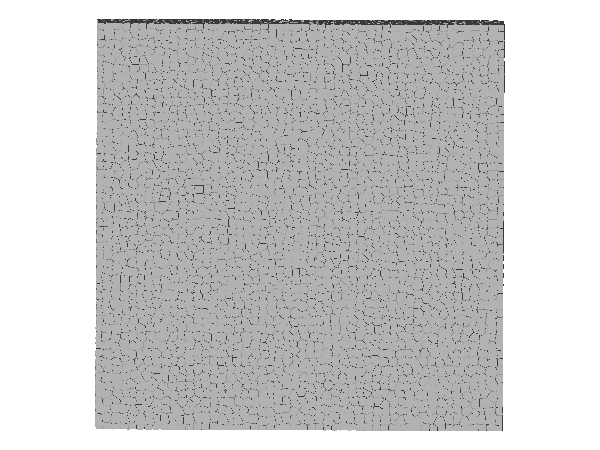
\includegraphics[width=.9\linewidth]{Files/exp_3D/DEF/A30X-1C_3_3ds.png}
    \caption{Intensified 100x100x100mm  \\ 0.6191\% Expansion}
    \end{subfigure}%
    %*******

    %*******
    \begin{subfigure}{.3\textwidth}
      \centering
      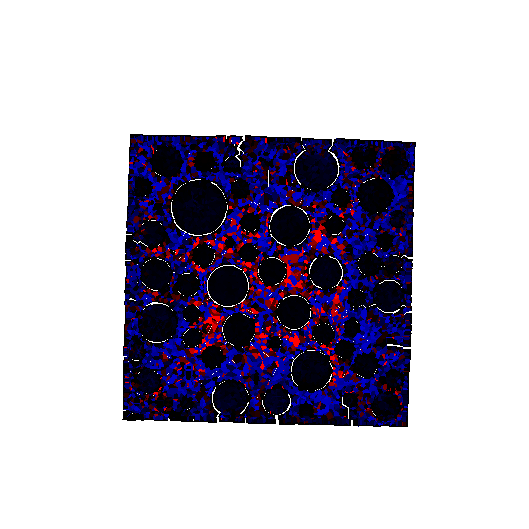
\includegraphics[width=.9\linewidth]{Files/exp_3D/DEF/A30X0C_3_stress.png}
    \caption{Intensified 50x50x50mm \\  0.5795\% Expansion}
    \end{subfigure}%
    %*******
    \begin{subfigure}{.3\textwidth}
      \centering
      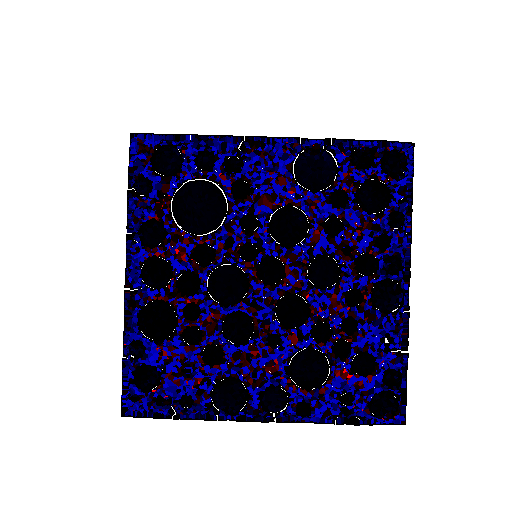
\includegraphics[width=.9\linewidth]{Files/exp_3D/DEF/A30X-5C_3_stress.png}
    \caption{Intensified 75x75x75mm  \\ 0.5118\% Expansion}
    \end{subfigure}
    %*******
    \begin{subfigure}{.3\textwidth}
      \centering
      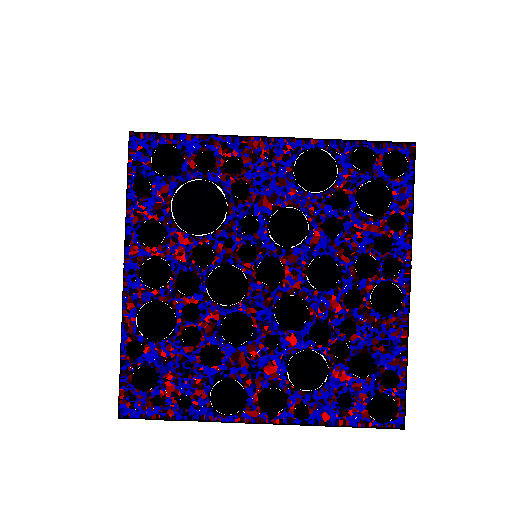
\includegraphics[width=.9\linewidth]{Files/exp_3D/DEF/A30X-1C_3_stress.png}
    \caption{Intensified 100x100x100mm \\  0.6191\% Expansion}
    \end{subfigure}%
    %*******

    %*******
    \begin{subfigure}{.3\textwidth}
      \centering
      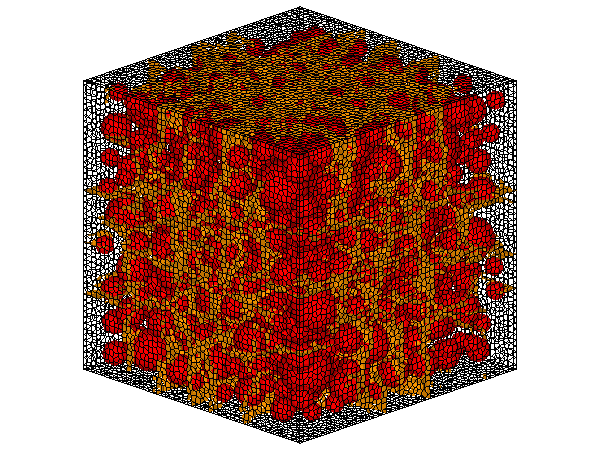
\includegraphics[width=.9\linewidth]{Files/exp_3D/DEF/A30X0C_3_c.png}
    \caption{Intensified 50x50x50mm \\  0.5795\% Expansion}
    \end{subfigure}%
    %*******
    \begin{subfigure}{.3\textwidth}
      \centering
      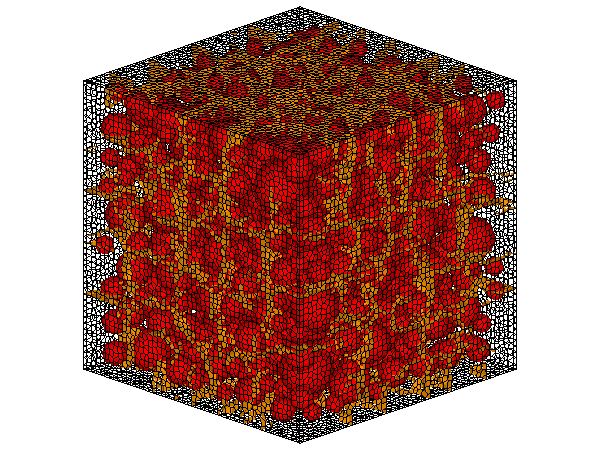
\includegraphics[width=.9\linewidth]{Files/exp_3D/DEF/A30X-5C_3_c.png}
    \caption{Intensified 75x75x75mm  \\ 0.5118\% Expansion}
    \end{subfigure}
    %*******
    \begin{subfigure}{.3\textwidth}
      \centering
      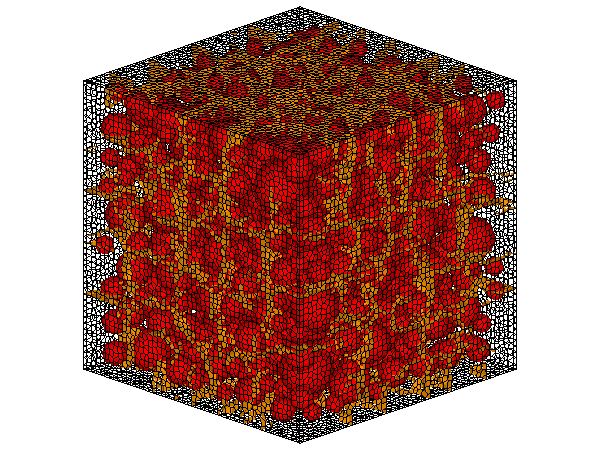
\includegraphics[width=.9\linewidth]{Files/exp_3D/DEF/A30X-1C_3_c.png}
    \caption{Intensified 100x100x100mm \\  0.6191\% Expansion}
    \end{subfigure}%
    %*******

  \caption{Comparing between different DEF Expansion Intensified Cases}
  \label{fig:DEF_X_compare}
\end{figure}


When examined closely of the intersection, it can be seen that no inner crack is happening in the paste for the uniformed expanding case, separation only happens between the surface of aggregate and paste, which is different with other 2 cases.

With expansion intensified in the inner part of concrete model, the compressive force concentrated in the inner part of the model, while outer parts are under tension. This unbalanced force generates cracks at the surrounding part of the concrete, preset as map cracking pattern at the surface view. This cracking pattern is also correlated with the observation form A.Awasthi in his investigation of DEF deteriorated  Indian concrete sleeper in 2016.

Figure here.
